%!TEX TS-program = xelatex
%!TEX encoding = UTF-8 Unicode

\documentclass[11pt,tikz,border=1]{standalone}
\usetikzlibrary{positioning,math}

\begin{document}
  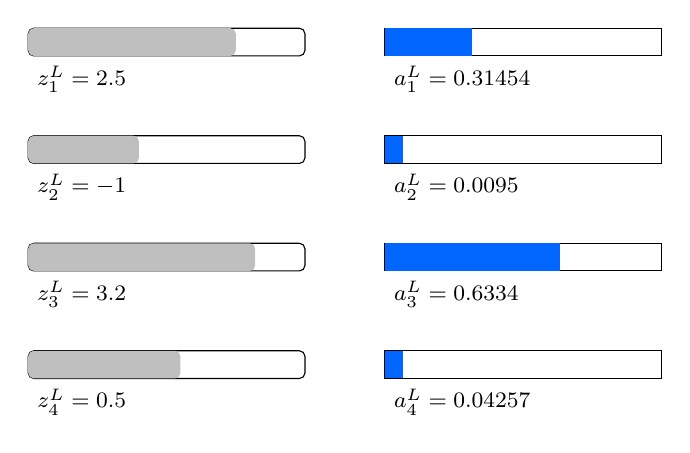
\begin{tikzpicture}[
    font=\footnotesize,
    base/.style={rectangle,draw,minimum width=100pt,minimum height=10pt},
    slidebar/.style={base,rounded corners=2pt},
    slidebarinner/.style={rectangle,fill=gray!50,rounded corners=2pt,minimum height=10pt},
    colorbar/.style={base},
    colorbarinner/.style={rectangle,minimum height=10pt,fill=blue!60!cyan}
  ]

  \node(s1) [slidebar] {};
  \node(z1) [below,anchor=north west] at (s1.south west) {$z^L_1 = 2.5$};

  \node(b1) [colorbar,right=of s1] {};
  %\node(a1) [below,anchor=north west] at (b1.south west) {$a^L_1 = 0.315$};

  \node(s2) [slidebar,below=of s1] {};
  \node(z2) [below,anchor=north west] at (s2.south west) {$z^L_2 = -1$};

  \node(b2) [colorbar,right=of s2] {};
  %\node(a2) [below,anchor=north west] at (b2.south west) {$a^L_2 = 0.009$};

  \node(s3) [slidebar,below=of s2] {};
  \node(z3) [below,anchor=north west] at (s3.south west) {$z^L_3 = 3.2$};

  \node(b3) [colorbar,right=of s3] {};
  %\node(a3) [below,anchor=north west] at (b3.south west) {$a^L_3 = 0.633$};

  \node(s4) [slidebar,below=of s3] {};
  \node(z4) [below,anchor=north west] at (s4.south west) {$z^L_4 = 0.5$};

  \node(b4) [colorbar,right=of s4] {};
  %\node(a4) [below,anchor=north west] at (b4.south west) {$a^L_4 = 0.043$};

	\tikzmath{
		function zsum(\za,\zb,\zc,\zd) {
    		return exp(\za) + exp(\zb) + exp(\zc) + exp(\zd);
		};
		function softmax(\n, \za, \zb, \zc, \zd) {
			return exp(\n) / zsum (\za, \zb, \zc, \zd);
		};
		function getslidewidth(\x) {
			return (\x + 5) * 10; 
		};
		\a = softmax(2.5, 2.5, -1, 3.2, 0.5);
	  	\wa = \a * 100;
	  	\wz = getslidewidth(2.5);
	  	{
  			\node(si1) [slidebarinner,minimum width=\wz pt,anchor=west] at (s1.west) {};
	  		\node(bi1) [colorbarinner,right=of s1,minimum width=\wa pt] {};
			\node(a1) [below,anchor=north west] at (b1.south west) {$a^L_1 = \a$};
	  	};
		\a = softmax(-1, 2.5, -1, 3.2, 0.5);
	  	\wa = \a * 100;
	  	\wz = getslidewidth(-1);
		{
  			\node(si2) [slidebarinner,minimum width=\wz pt,anchor=west] at (s2.west) {};
	  		\node(bi2) [colorbarinner,right=of s2,minimum width=\wa pt] {};
			\node(a2) [below,anchor=north west] at (b2.south west) {$a^L_2 = \a$};
		};
		\a = softmax(3.2, 2.5, -1, 3.2, 0.5);
	  	\wa = \a * 100;
	  	\wz = getslidewidth(3.2);
  		{
  			\node(si3) [slidebarinner,minimum width=\wz pt,anchor=west] at (s3.west) {};
	  		\node(bi3) [colorbarinner,right=of s3,minimum width=\wa pt] {};
  			\node(a3) [below,anchor=north west] at (b3.south west) {$a^L_3 = \a$};
  		};
		\a = softmax(0.5, 2.5, -1, 3.2, 0.5);
	  	\wa = \a * 100;
	  	\wz = getslidewidth(0.5);
  		{
  			\node(si4) [slidebarinner,minimum width=\wz pt,anchor=west] at (s4.west) {};
	  		\node(bi4) [colorbarinner,right=of s4,minimum width=\wa pt] {};
  			\node(a4) [below,anchor=north west] at (b4.south west) {$a^L_4 = \a$};
  		};
	}

  \end{tikzpicture}
\end{document}
